\section*{A-4. Artificial neural network (ANN)}

The solution is based on \cite{Le2021}.

The original ANN use four seperate classifier for four class respectively. Since 2nd classifier only has 1 training sample, we need to restructure this model such that each classifier can have acceptable number of training samples. We do this by changing this "fat" ANN to "deep" ANN, and creating some new type of classifiers.

\begin{figure}[ht!]
	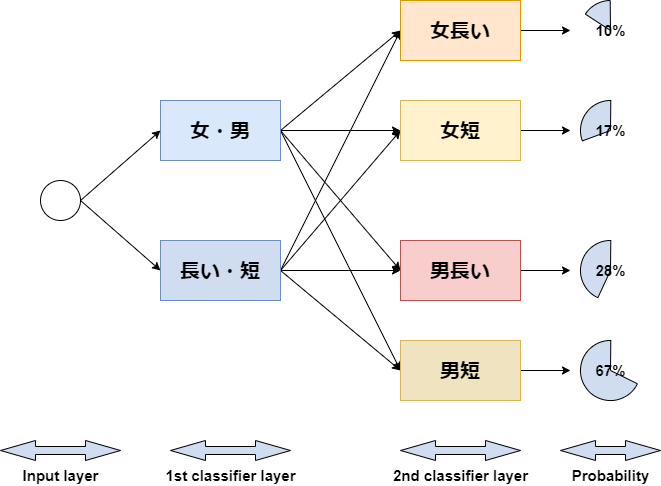
\includegraphics[scale=0.7]{./Images/ANN}
	\caption{Architecture of improving classifiers model}
	\label{fig:ANN1}
\end{figure}

The new model is shown as Image \ref{fig:ANN1}. Since we have enormous number of samples of girl/boy class and long/short hair class, first we train two seperate classifiers for these two pair class. Now we do transfer learning by connecting trained 1st classifier layer with 2nd classifier layer. Since the 1st layer has knowlegde about girl/boy pair class and long/short pair class, it can transfer that information directly to 2nd layer. The 2nd layer now only need to find a way to connect results from two classifier in 1st layer and return a probability a sample belong to a class.

The "deep" ANN can use the knowledge from lower layers and build up more complicated structure in higher layers. We can also utilise the pretrained module/layer and corporate them to our new model so we can overcome the case that some class has less number of samples.